\lecture{2009-12-08}

\subsection{Regeln von L'Hospital}

unbestimmte Ausdrücke der Form $\frac 0 0$, $\frac \infty \infty$, $0 \cdot \infty$, $\ldots$ $\approx$ 1680 (Bernoulli)
\begin{example}\[ \liminfty[x]{\frac{\sin x} x} \]\end{example}

\noindent Hilfsmittel dazu: 2. Mittelwertsatz der Differentialrechnung
\begin{theorem}
  $f,g: \left[a,b\right] \to \mathbb R$ stetig und differenzierbar mit $g'(x) \neq 0$
  \[ g(a) \neq g(b) \implies \exists x_0: \frac{f(b)-f(a)}{g(b)-g(a)}=\frac{f'(x_0)}{g'(x_0)}  \]
\end{theorem}
\begin{note}
  nach 1. Mittelwertsatz
  \begin{equation*} \cfrac{\frac{f(b)-f(a)}{b-a}}{\frac{g(b)-g(a)}{b-a}} = \frac{f'(x_1)}{g'(x_2)} \end{equation*}
  mit $a < x_1, x_2 < b$, aber nicht $x_1 = x_2$
\end{note}
\begin{proof}
  Hilfsfunktion: $h(x) = f(x) - \frac{f(b)-f(a)}{g(b)-g(a)} \cdot (g(x)-g(a))$ stetig, differenzierbar
  \[
    \left.\begin{array}{r}h(a) = f(a)\\h(b)=f(a)\end{array}\right\} \leadsto \text{ Satz von Rolle: } \exists \textcolor{blue}{x_0}: h'(x_0) = 0
  \]
  \[ h'(x) = f'(x) - \frac{f(b)-f(a)}{g(b)-g(a)} \cdot g'(x) \]
  \[ \textcolor{blue}{x_0}: h'(x_0) = 0 = f'(x_0) - \frac{f(b)-f(a)}{g(b)-g(a)} \cdot g'(x_0) \]
  \[ \implies \frac{f(b)-f(a)}{g(b)-g(a)} = \frac{f'(x_0)}{g'(x_0)} \]
\end{proof}

\begin{theorem}[Regeln von L'Hospital]\label{theorem:hospital} Aus $f, g: \left]a,b\right[ \to \mathbb R$ differenzierbar mit $g'(x) \neq 0$, außerdem
  \begin{equation*} f(x), g(x) \xrightarrow[x \rightarrow a]{} 0 \text{ oder } f(x), g(x) \xrightarrow[x \rightarrow a]{} \infty \end{equation*}
  folgt:

  Falls der Grenzwert $\lim_{x \rightarrow a} \frac{f'(x)}{g'(x)}$ existiert, dann existiert auch der Grenzwert $\lim_{x \rightarrow a} \frac{f(x)}{g(x)}$, wobei
  \[ \lim_{x \rightarrow a} \frac{f(x)}{g(x)} = \lim_{x \rightarrow a} \frac{f'(x)}{g'(x)} \]
\end{theorem}
\begin{note}Nicht zu verwechseln mit der Quotientenregel! Zähler und Nenner werden getrennt voneinander differenziert.\end{note}
\begin{example}
  \begin{itemize}
    \item $\displaystyle\lim_{x \rightarrow 0} \underbrace{\left(\frac{\sin x} x\right)}_{\text{Form }\frac 0 0} =
      \lim_{x \rightarrow 0} \left(\frac{\cos x} 1\right) = 1$
    \item nützliche Umformungen
      \begin{footnotesize}\begin{align*}
        f(x) \cdot g(x) \text{ hat Form } 0 \cdot \infty &\implies f(x) \cdot g(x) = \frac{f(x)}{\frac 1 {g(x)}} \text{ hat Form } \frac 0 0 \\
        f(x) - g(x) \text{ hat Form } \infty - \infty &\implies f(x) \cdot g(x) \cdot \left( \frac 1 {f(x)} - \frac 1 {g(x)} \right) \text{ hat Form } \frac 0 0 \text { oder } \frac\infty\infty \\
      \end{align*}\end{footnotesize}
    \item
      \begin{align*}
        \lim_{x \rightarrow 0} \underbrace{\left( \frac 1 x - \frac 1 {\sin x} \right)}_{\text{Form } \infty - \infty}
        &= \lim_{x \rightarrow 0} \underbrace{\left( \frac{\sin x - x}{x \cdot \sin x} \right)}_{\text{Form } \frac 0 0} \\
        &= \lim_{x \rightarrow 0} \underbrace{\left( \frac{\cos x - 1}{x \cdot \cos x + \sin x} \right)}_{\text{Form } \frac 0 0} \\
        &= \lim_{x \rightarrow 0} \left( \frac{-\sin x}{2 \cdot \cos x - x\cdot \sin x} \right) \\
        &= \frac 0 2 = 0
      \end{align*}
  \end{itemize}
\end{example}

\subsubsection*{Nachtrag: Differentiation der $\euler$-Funktion $\euler^x$}

Einführung $\euler^x$ als Folgengrenzwert:
\begin{equation*}
  \euler^x = \liminfty{\left( 1+\frac x n\right)^n}
\end{equation*}
Definition $g(x) = \liminfty{\left( 1+\frac x n\right)^n}$, stetig differenzierbar
\begin{align*}
  \implies g'(x) &= \frac n n \cdot \left( 1+\frac x n\right)^{n-1} = \left( 1+\frac x n\right)^{n-1} \\
  &= \left( 1+\frac x n\right)^{-1}\cdot \left( 1+\frac x n\right)^{n} \\
  &= \left( 1+\frac x n\right)^{-1}\cdot g(x) \\
  &\xrightarrow[n \rightarrow \infty]{x: \text{ fest}} g(x)
\end{align*}

\begin{note}
  $\euler$-Funktion ist so gebaut, dass Ableitung $=$ Funktion $\leadsto$ gewöhnliche Differentialgleichung:
  \begin{align*}
    \dot y = y &\implies y(t) = c\cdot \euler^t \\
    \lambda \in \mathbb R\quad \dot y = \lambda y &\implies y(t) = c \cdot \euler^{\lambda t}
  \end{align*}
  (wegen $\frac\diff{\diff t} \euler^{h(t)} = h'(t)\cdot\euler^{h(t)}, h(t) = \lambda t$)

\end{note}

\subsection{Kurvendiskussion $y = f(x)$}

\begin{enumerate}
  \item Definitionsbereich, Wertebereich
  \item Symmetrien (gerade, ungerade)
  \item Stetigkeit, Polstellen
  \item Nullstellen% (siehe \todo{Referenz auf 7.8 bzw. 2.3.8})
  % LH: Referenz wäre sinnlos, in 7.8 geht es um Umkehrfunktionen
  \item $f'$ berechnen, $f' = 0$ Nullstellen
  \item Extremwerte: innere Extrema, Randextrema, Monotoniebereiche
  \item $f''$ berechnen, $f'' = 0$ Nullstellen
  \item Wendepunkte, konvexe/konkave Bereiche
  \item asymptotisches Verhalten $x \rightarrow \pm\infty$
  \item Graph
\end{enumerate}

\subsection{Gewöhnliche Differentialgleichungen -- 2. Teil}

\begin{wrapfigure}{r}[1cm]{.4\textwidth}
  \centering
  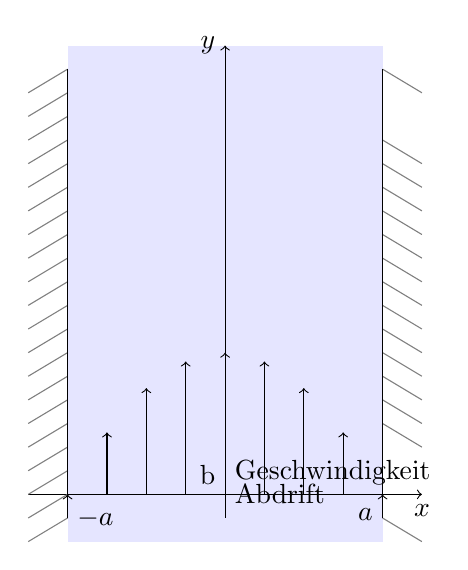
\begin{tikzpicture}[scale=0.5,y=0.6cm]
    \fill[color=blue!10] (-4,-2) -- (-4,19) -- (4,19) -- (4,-2);

    % x-Achse
    \draw[->] (-5,0) -- (5,0) node[below] {$x$};
    \draw (-4,0.2) -- (-4,-0.2) node[below right] {$-a$};
    \draw (4,0.2) -- (4,-0.2) node[below left] {$a$};

    % y-Achse
    \draw[->] (0,-1) -- (0,19) node[left] {$y$};

    % Landmarkierung
    \foreach \x in {-1,...,18}
      \draw[color=gray] (-5,\x-1) -- (-4.0,\x);

    \foreach \x in {-1,3,4,...,15,18}
      \draw[color=gray] (5,\x-1) -- (4,\x);

    % Flussgrenzen
    \draw (-4,-1) -- (-4,18);
    \draw (4,-1) -- (4,18);

    % Flussgeschwindigkeitsfunktion
    \draw[domain=-4:4] plot [id=flussgeschw, samples=50] function {6*(1-(x**2)/(4**2))} node[above right] {Geschwindigkeit};
    % Geschwindigkeitsvektoren
    \foreach \x/\y in {-4/0, -3/2.625, -2/4.5, -1/5.625, 0/6, 1/5.625, 2/4.5, 3/2.625, 4/0}
      \draw[->] (\x,0) -- (\x,\y);

    % Abdriftsfunktion
    \draw[domain=-4:4] plot [id=abdrift, samples=50] function {3*(x-(x**3)/(3*4**2))+8} node[right] {Abdrift} node[above left] {b};
  \end{tikzpicture}
\end{wrapfigure}
% Derbster Hack aller Zeiten:
$ $ % Ich weiß nicht, was hier passiert. Anders geht es aber nicht.
% siehe http://www.cis.hut.fi/ntvuok/scripts.php --LH
\begin{example}[Hund springt in Eisbach und driftet ab]\flush
  \begingroup
  \newcommand{\kmh}{\ensuremath{\,\textstyle \frac{\text{km}}{\text{h}}}}
  \begin{itemize}
    \item $v_0$ maximale Geschwindigkeit des Wasser
      \begin{equation*} v_0 = 6 \kmh \end{equation*}
      Wahl: Parabelprofil
      \begin{equation*} v_\text{F}(x) = v_0 \cdot \left( 1 - \frac{x^2}{a^2} \right) \end{equation*}
      \begin{equation*} v(a) = v(-a) = 0 \end{equation*}
    \item Hund: konstante Eigengeschwindigkeit
      \begin{align*}
        v_H &= 2 \kmh \\
        v_H &\parallel \text{$x$-Achse}
      \end{align*}
  \end{itemize}
  \par
  \begin{itemize} % hack
    \item Fragen: Welche Bahn schwimmt der Hund? Wie groß ist seine Abdrift $b$?
      \begin{equation*} \left. \tan \alpha = \frac{v_\text{F}}{v_\text{H}} = y'(x) \quad\right\rangle\quad y'(x) = \frac{v_0}{v_\text{H}} \cdot \left( 1 - \frac{x^2}{a^2}\right)\end{equation*}
    \item Erraten der Lösung
      \begin{equation*}
      y(x) = c + \frac{v_0}{v_\text{H}} \cdot \left( x - \frac{x^3}{3a^2}\right)
      \end{equation*}
    \item Abdrift
      \begin{align*}
        b = \underbrace{y(a)}_{\parbox{16mm}{\centering\scriptsize landet der Hund}} -\underbrace{y(-a)}_{\parbox{16mm}{\centering\scriptsize startet der Hund}} &= \ds\frac{v_0}{v_\text{H}} \cdot \underbrace{\left( \left( a - \frac{a^3}{3a^2}\right) - \left( -a + \frac{a^3}{3a^2}\right) \right)}_{2a - \frac 2 3 a} \\
        &= \ds\frac 4 3 \cdot \frac{v_0}{v_\text{H}}\cdot  a
      \end{align*}
      in Zahlen:
      \begin{equation*}
        b = \frac 4 3 \cdot \frac {6 \kmh}{2 \kmh} \cdot 4 \,\text{m} = 16 \,\text{m}
      \end{equation*}
  \end{itemize}
  \endgroup
\end{example}

